%% F1
\begin{figure*}[ht]
  \begin{subfigure}{.315\textwidth}
    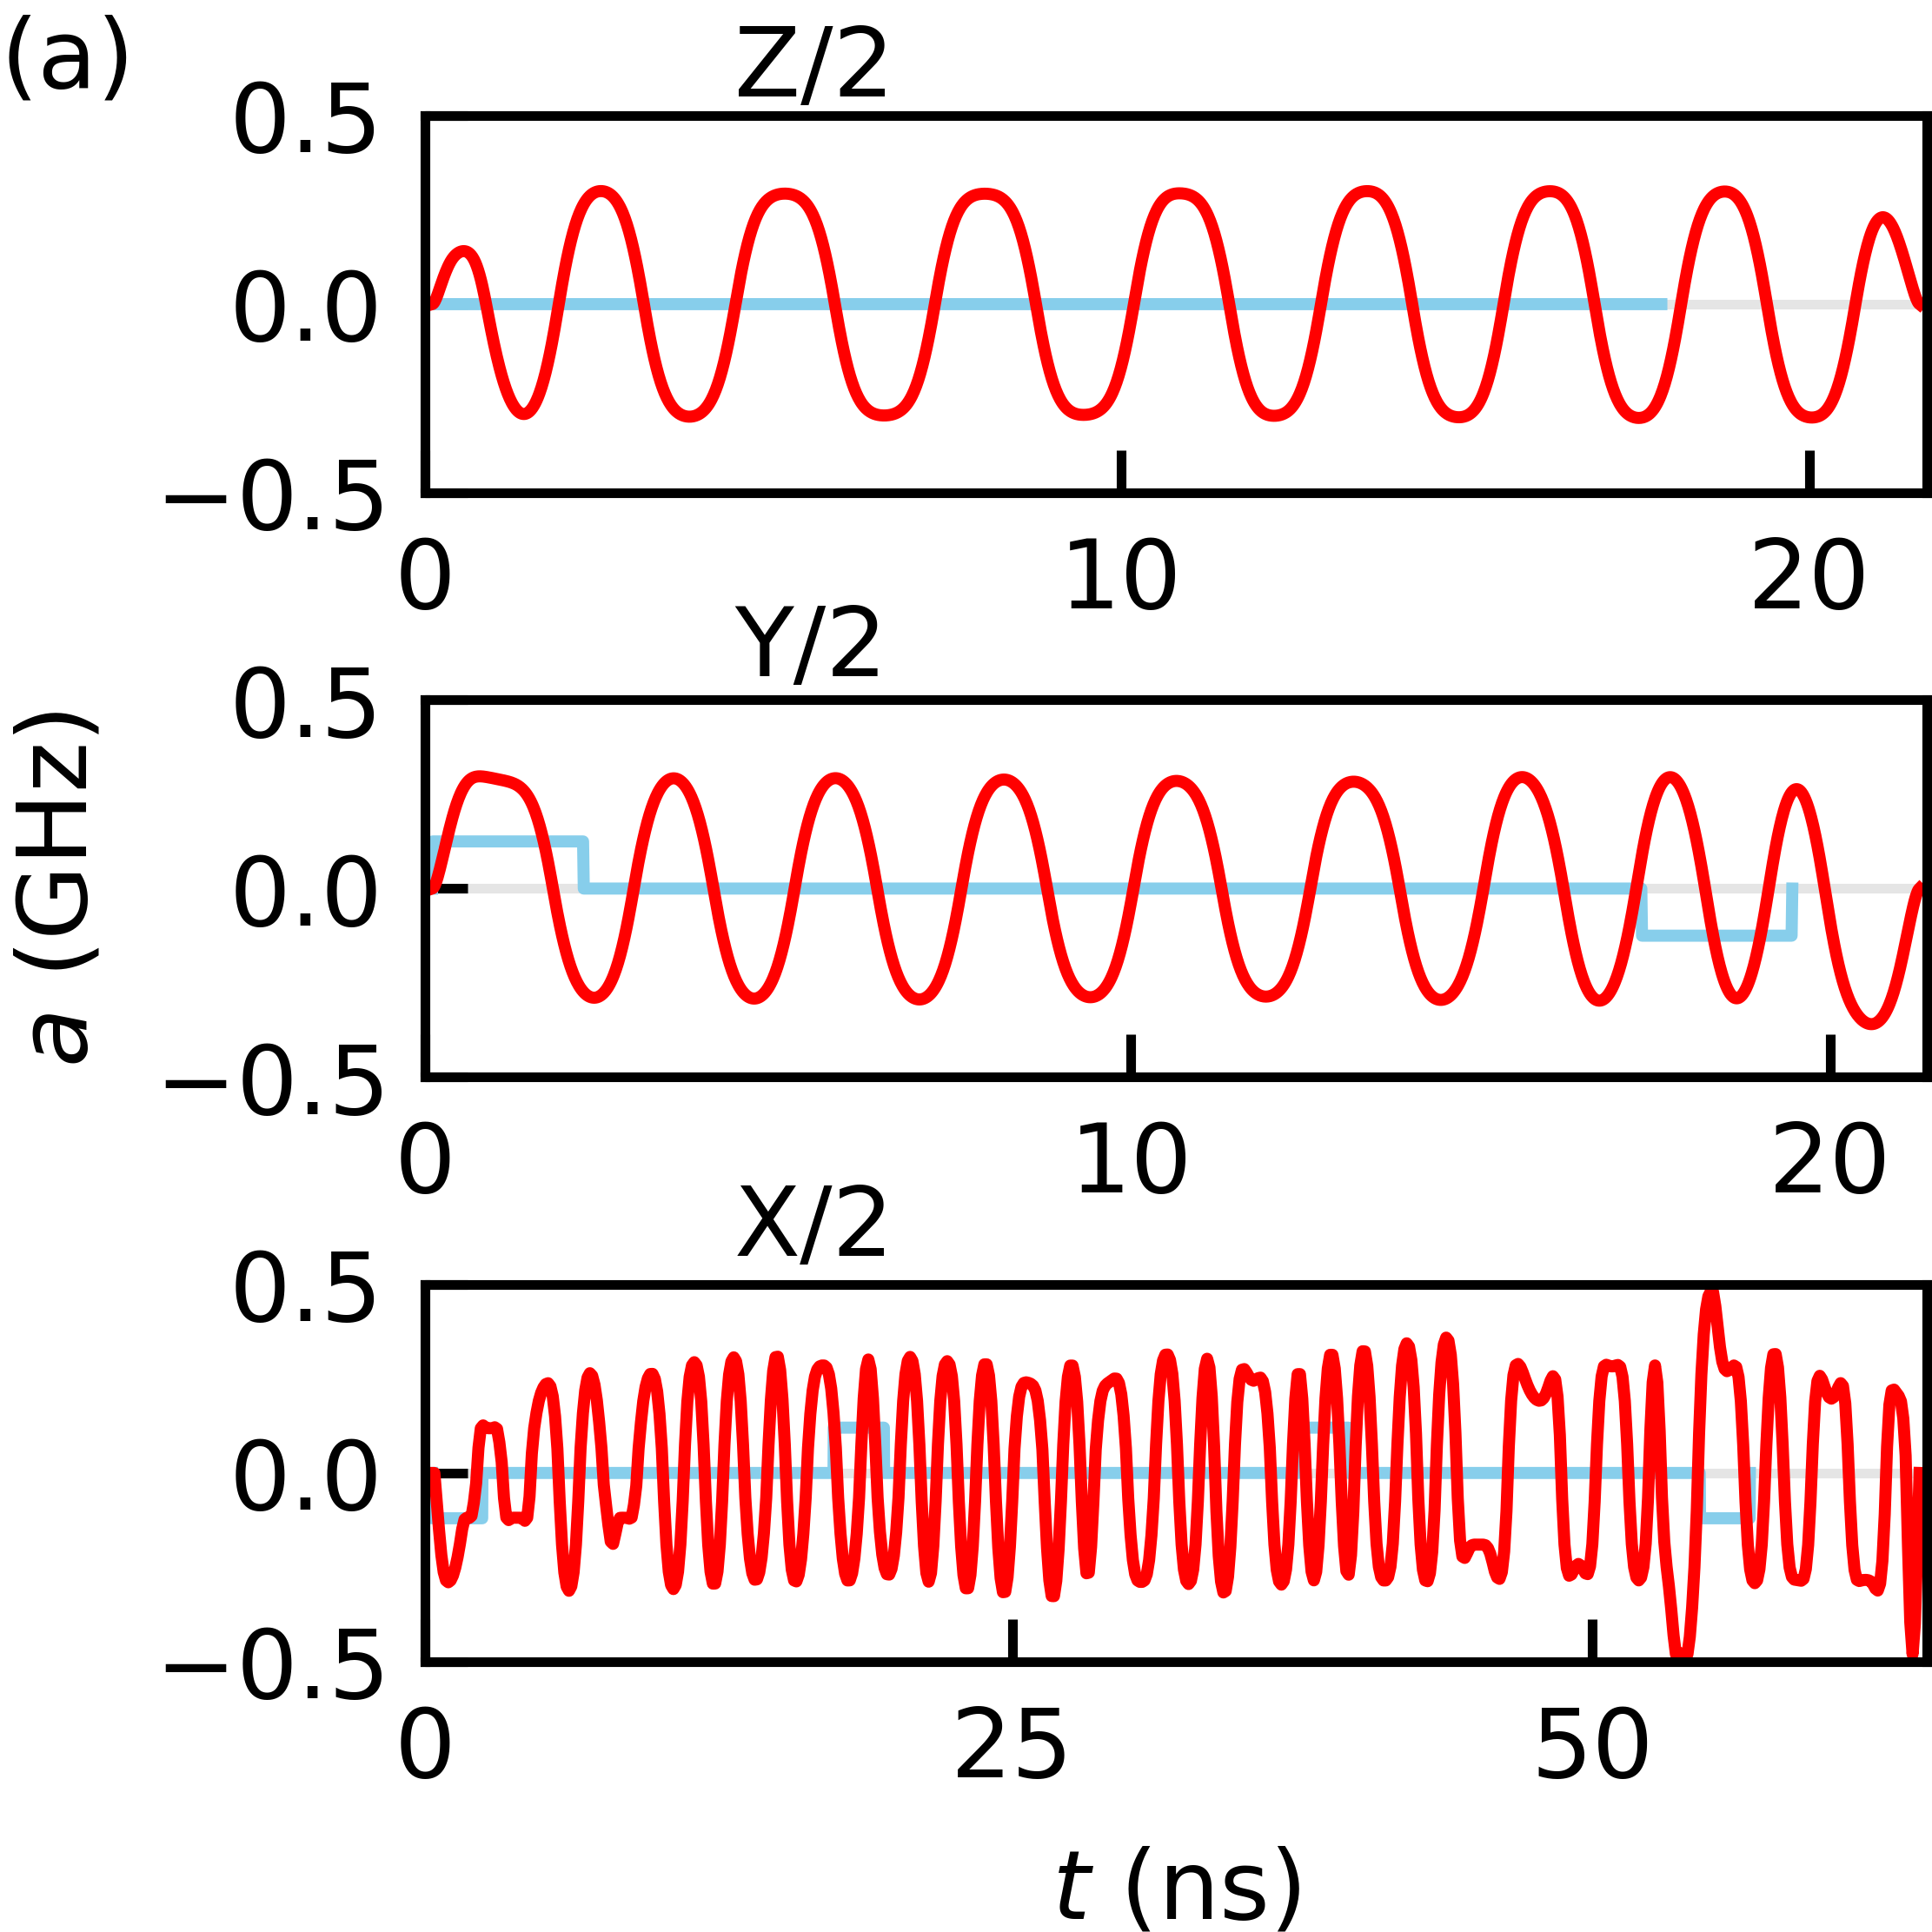
\includegraphics[width=\linewidth]{assets/f1a.png}
    \caption{\label{fig:longitudea}}
  \end{subfigure}\hfill
  \begin{subfigure}{.23\textwidth}
    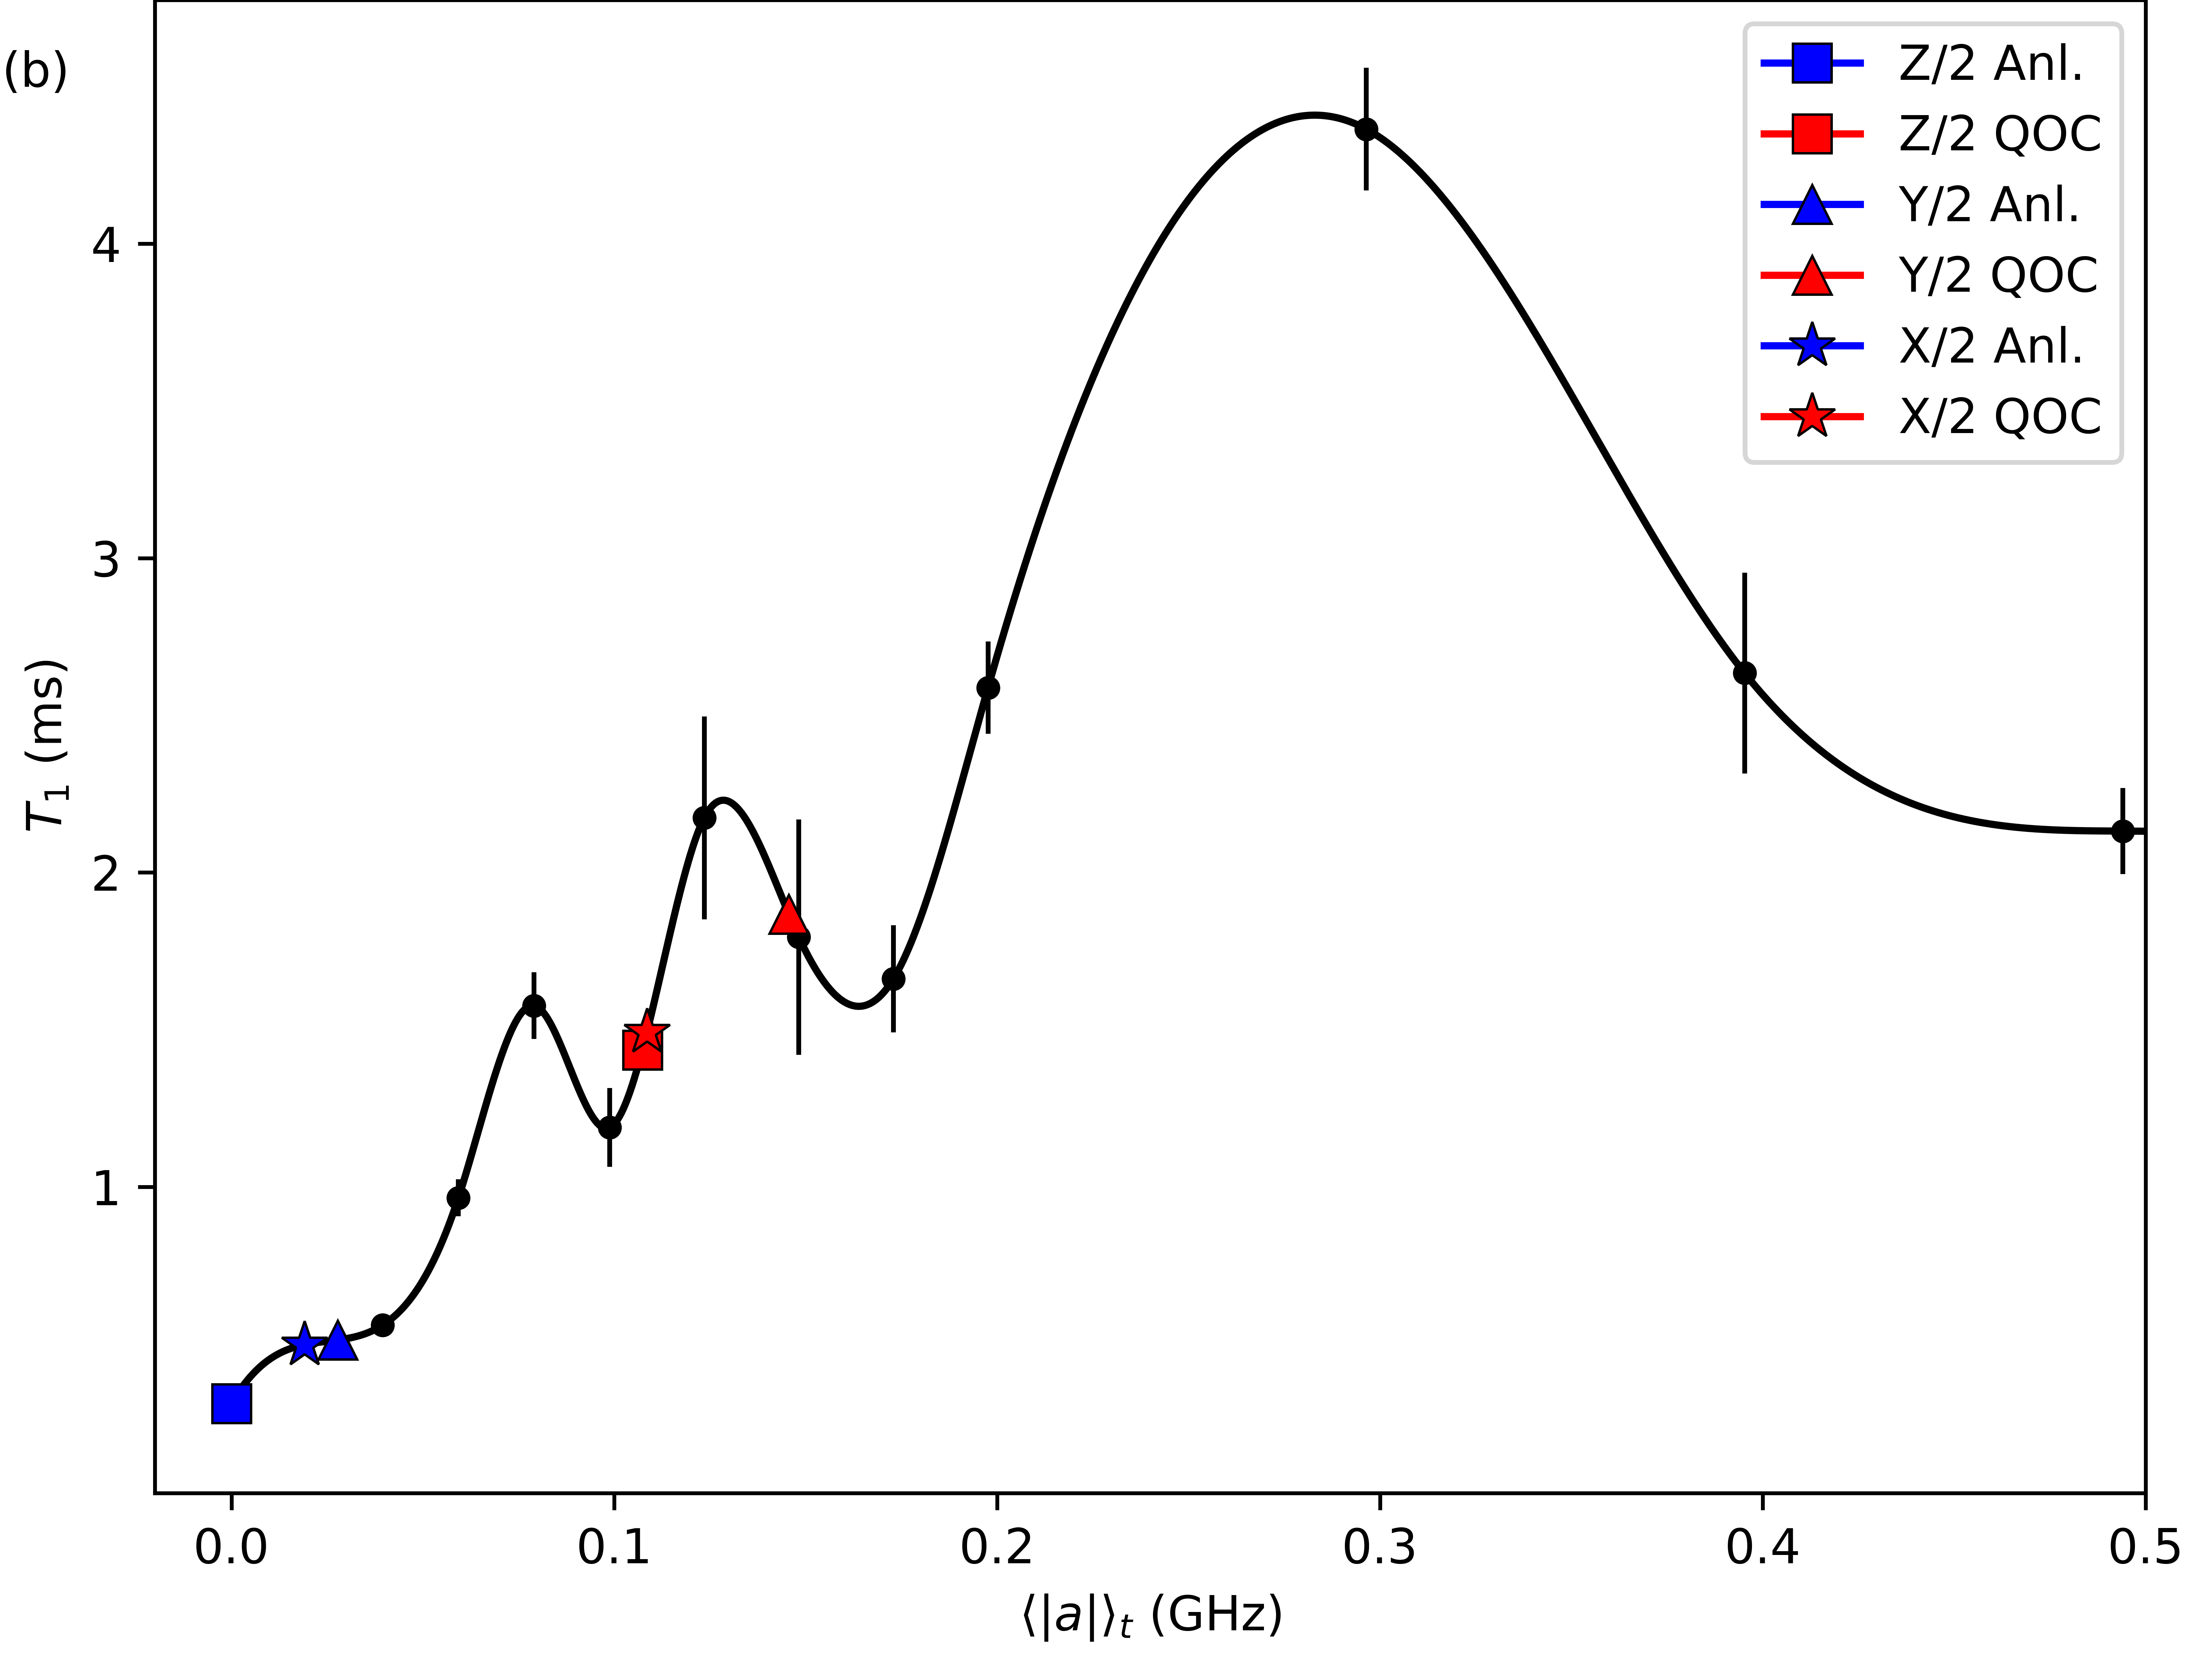
\includegraphics[width=\linewidth]{assets/f1b.png}
    \caption{\label{fig:longitudeb}}
  \end{subfigure}\hfill
  \begin{subfigure}{.4\textwidth}
    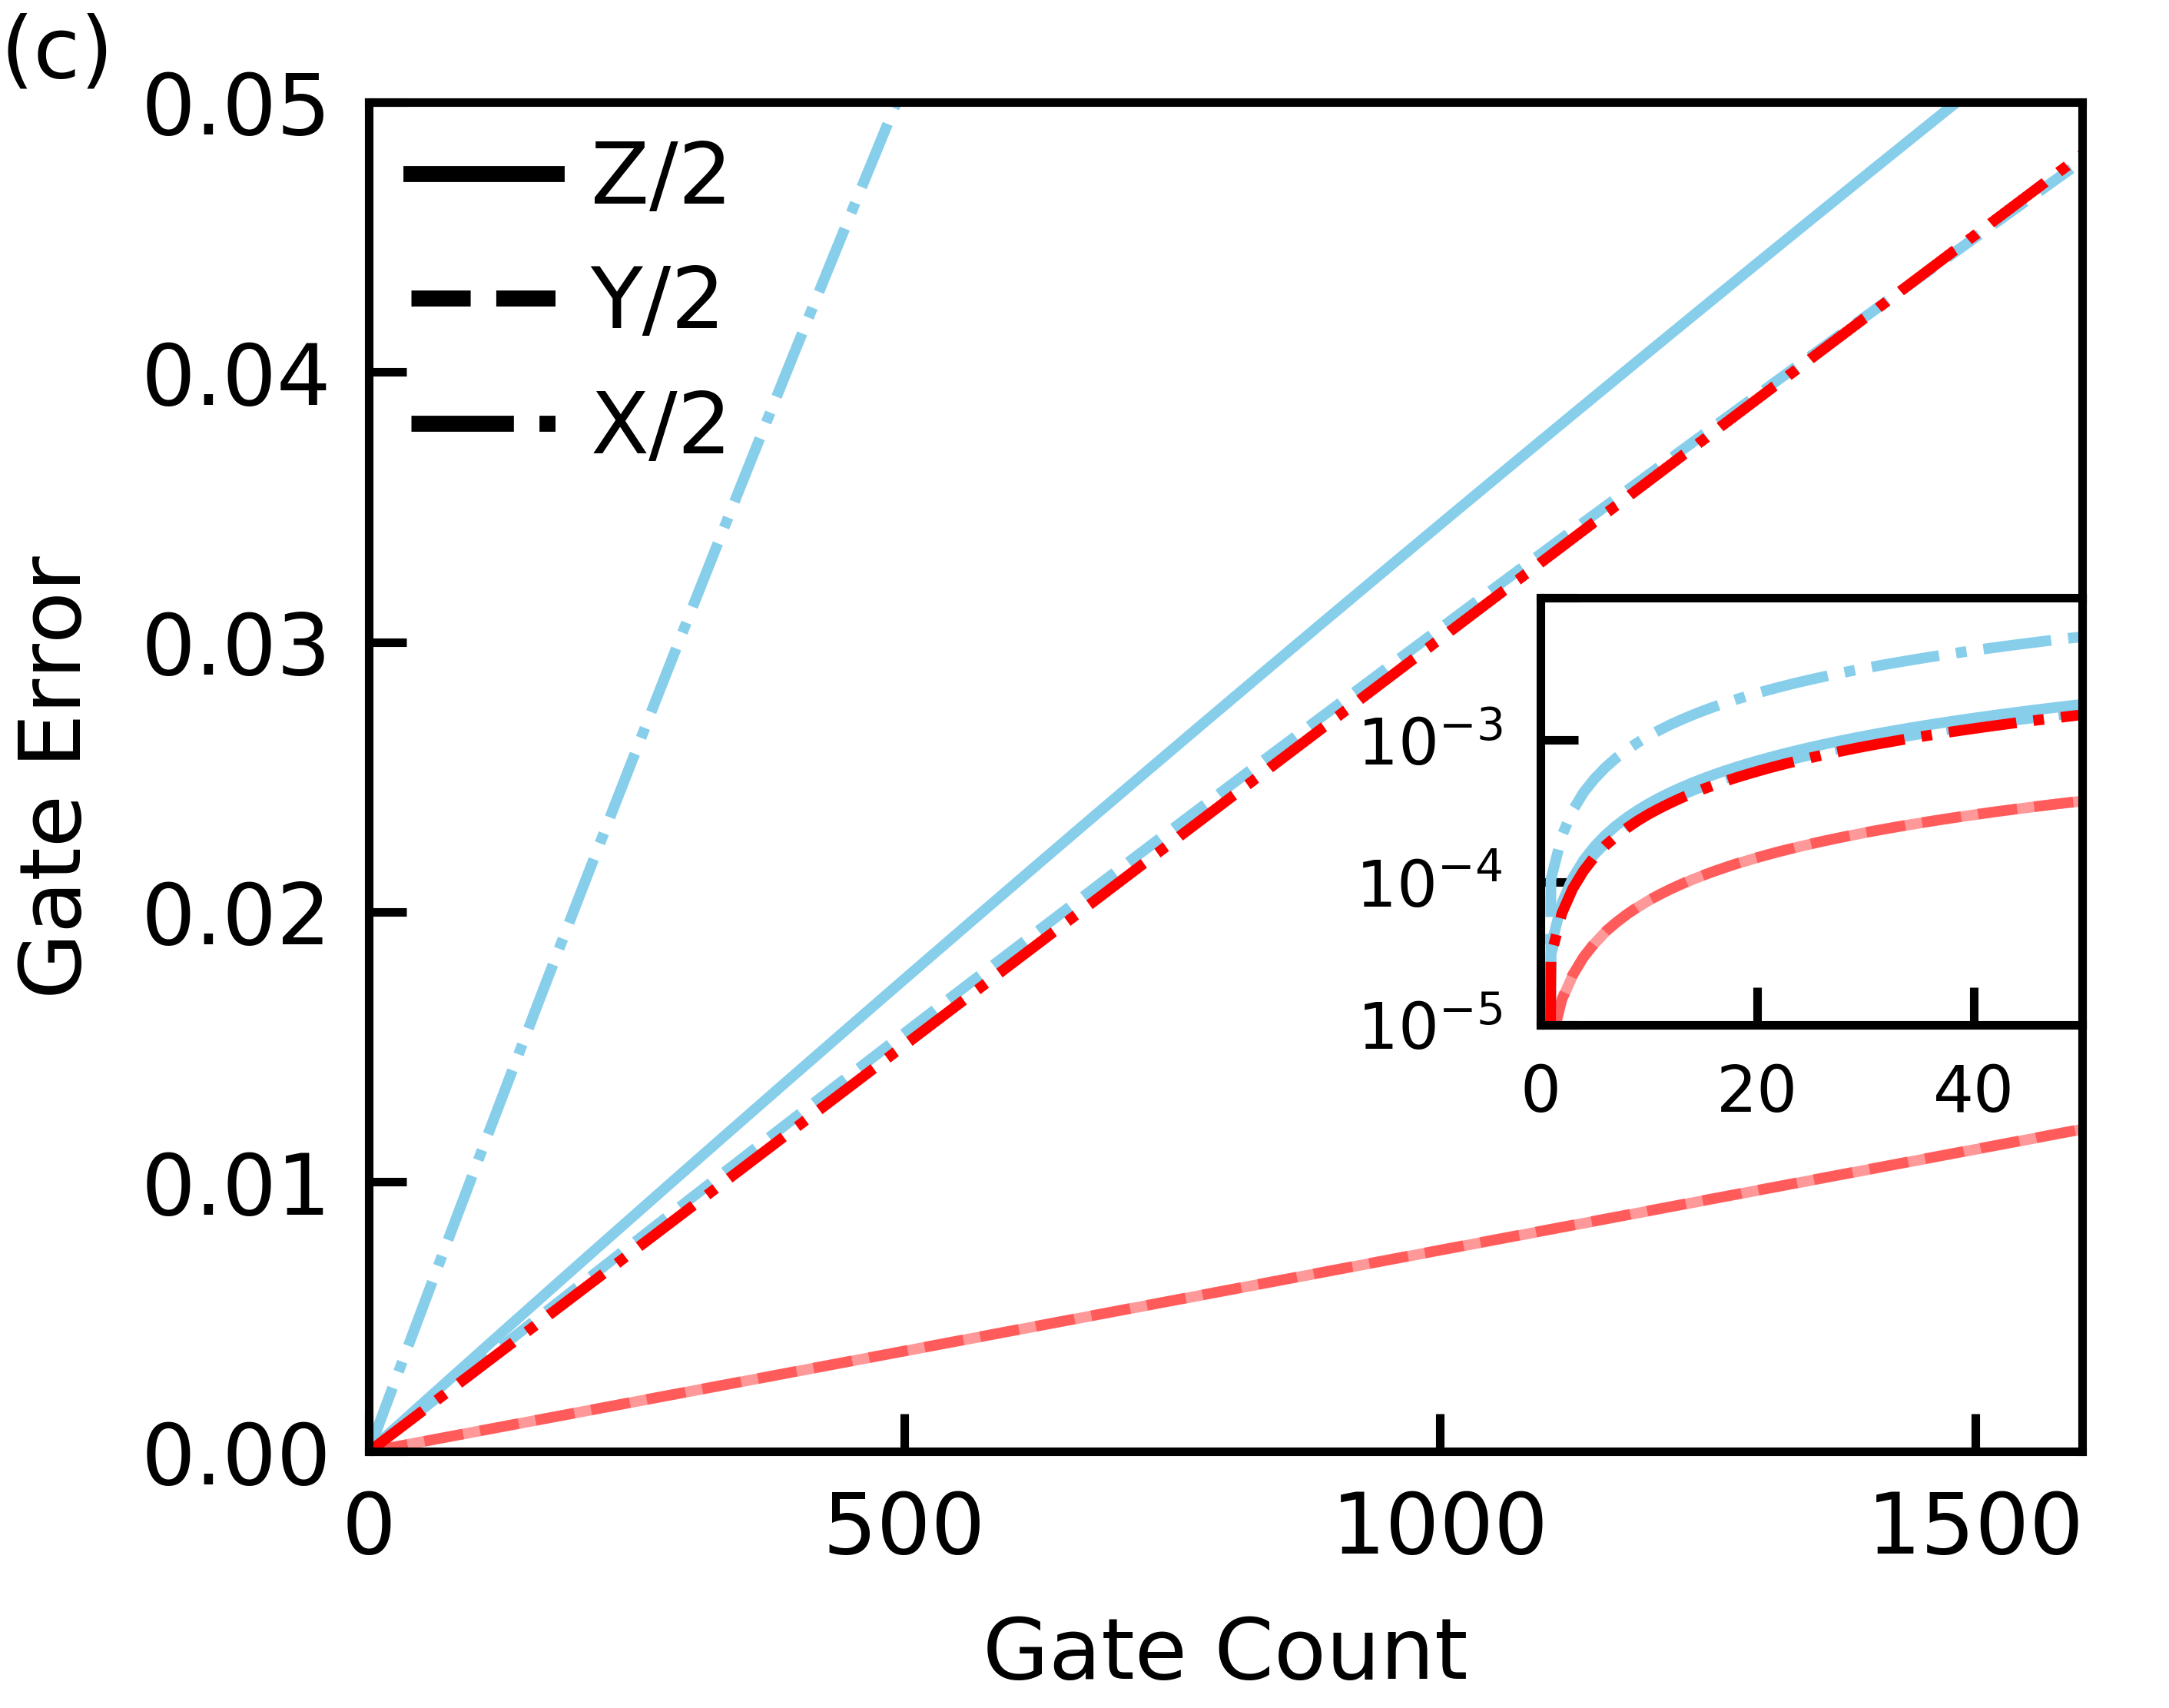
\includegraphics[width=\linewidth]{assets/f1c.png}
    \caption{\label{fig:longitudec}}
  \end{subfigure}
  \caption{
    (a) Flux pulses for the numerical gates (dark blue)
    and the analytic gates (light pink).
    (b) $T_{1}$ interpolation function used in optimization. Circle markers
    indicate measured $T_{1}$ times. Non-circle markers
    are plotted at the time-averaged 
    absolute flux and the time-averaged $T_{1}$ time for each pulse.
    (c) Cumulative gate errors due to depolarization as a function of the
    number of gates applied.
    Cumulative gate errors for the numerical $Z/2$ and $Y/2$ gates
    are indistinguishable. Inset shows log-scaled cumulative gate errors
    for small gate counts.
  }
  \label{fig:longitude}
\end{figure*}

\section{QOC for the Fluxonium \label{sec:fluxonium}}
In the following, we optimize quantum gates
for the superconducting fluxonium qubit--a promising
building block for quantum computers due to its high
coherence times
\cite{earnest2018realization, lin2018demonstration,
  manucharyan2009fluxonium, nguyen2019high,
  zhang2020universal}.
In this section, we outline the base optimization problem,
which we extend in subsequent sections to account
for experimental error channels.
To high accuracy, we approximate the Hamiltonian near the flux-frustration
point as a two-level system:
\begin{align}
  H/h &= f_{q} \frac{\sigma_{z}}{2} + a(t) \frac{\sigma_{x}}{2},
  \label{eq:hamiltonian}
\end{align}
where $f_{q}$ is the qubit frequency at the flux-frustration point,
$a(t)$ is the flux offset from the flux-frustration point,
$h$ is Planck's constant, and $\sigma_{z}, \sigma_{x}$
are Pauli matrices. We optimize $X/2$,
$Y/2$, and $Z/2$ gates (unitary transformations)
for the fluxonium presented in \cite{zhang2020universal},
and compare them to the analytically constructed gates for
that device.

First, we outline the constraints for the fluxonium gate problem.
All gates presented in this work satisfy these constraints to
a tolerance of $\sim 10^{-8}$.
Casting this problem as a multi-state transfer, the initial conditions on
the states are $\ket*{\psi^{0}_{1}} = \ket*{0}$, $\ket*{\psi^{1}_{1}} = \ket*{1}$
\eqref{eq:istate_con}
where the superscript is an index $i \in \{0, 1\}$,
and the subscript indicates the knot point $k = 1$.
The states at the final knot point are constrained to be
the target states $\ket*{\psi^{i}_{N}} = U \ket*{\psi^{i}_{1}} \ \forall \ i$
\eqref{eq:tstate_con} where $U = X/2, Y/2, Z/2$ is the desired gate.
Furthermore, we impose the normalization constraint
${\lvert \braket*{\psi^{i}_{k}}{\psi^{i}_{k}} \rvert}^{2} = 1 \ \forall \ i,k$
\eqref{eq:statenorm_con}
to ensure the solver does not take advantage of discretization errors in numerical integration.
To refer to the discrete moments of the flux, we introduce the notation
$\int^{t_{k}}_{t_{1}} a(t) \ \mathrm{d}t \equiv \int_{t} a_{k}$,
$a(t_{k}) \equiv a_{k}$,
$\pdv*[n]{a(t)}{t} \lvert_{t = t_{k}} \equiv \partial^{n}_{t} a_{k}$.
We impose the zero net flux constraint $\int_{t} a_{N} = 0$
\eqref{eq:znf_con}
which mitigates the inductive drift ubiquitous in flux-bias lines
\cite{battistel2019fast, krantz2019quantum, zhang2020universal}.
The flux is constrained by $\lvert a_{k} \rvert \leq 0.5 \ \textrm{GHz} \ \forall \ k$
\eqref{eq:amp_con}.
Above $0.5$ GHz, we observe excitation out of the first two levels, disallowing the
approximation \eqref{eq:hamiltonian}.
We also enforce the boundary condition $a_{1} = a_{N} = 0$ \eqref{eq:bound_con}
so the gates may be concatenated arbitrarily. Additionally,
we have the initial condition $\int_{t} a_{1} = \partial_{t} a_{1} = 0$
\eqref{eq:ic_con}.

Next, we introduce the augmented control and augmented state:
\begin{equation}
  \begingroup
  \renewcommand*{\arraystretch}{1.3}
  u_{k} = \begin{bmatrix} \partial^{2}_{t} a_{k} \end{bmatrix}, \quad
  x_{k} = \begin{bmatrix} \ket{\psi^{0}_{k}} \\ \ket{\psi^{1}_{k}}
    \\ \int_{t} a_{k} \\ a_{k} \\ \partial_{t} a_{k} \end{bmatrix}.
  \endgroup
  \label{eq:astatecontrols}
\end{equation}
The variables in the augmented state are obtained from the decision variable
in the augmented control
via coupled, first-order, differential equations, which are integrated in the 
discrete dynamics function \eqref{eq:dyn_con}.
We integrate the states according to the TDSE \eqref{eq:tdse} and the
fluxonium Hamiltonian \eqref{eq:hamiltonian}.
The ALTRO implementation we use does not currently
support complex numbers, so we repesent the states
in the isomorphism $\mathcal{H}(\mathbb{C}^{n})
\cong \mathcal{H}(\mathbb{R}^{2n})$ given in \cite{leung2017speedup},
\begin{equation}
  H \ket{\psi} \cong \begin{bmatrix} H_{\textrm{re}} & -H_{\textrm{im}}
    \\ H_{\textrm{im}} & H_{\textrm{re}}\end{bmatrix}
  \begin{bmatrix} \ket{\psi}_{\textrm{re}} \\ \ket{\psi}_{\textrm{im}}\end{bmatrix}.
  \label{eq:isomorphism}
\end{equation}

The cost function at each knot point is
$\ell_{k}(x_{k}, u_{k}) = (x_{k} - x_{f})^{T} Q_{k} (x_{k} - x_{f}) + u^{T}_{k} R_{k} u_{k}$
where $Q_{k}$ and $R_{k}$ are diagonal matrices we supply.
The $Q_{k}$ term
penalizes deviations from the final augmented state $x_{f}$,
which is given by the constraints we have imposed on
$\ket*{\psi^{i}_{N}}$, $\int_{t} a_{N}$, and $a_{N}$ in addition to
$\partial_{t} a_{f} = 0$.
The $R_{k}$ term penalizes the norm of $\partial^{2}_{t} a_{k}$,
smoothing the flux to mitigate high-frequency AWG transitions.
Stated succinctly, the optimization problem takes the form:
\begin{mini!}[2] 
  {x_{1:N}, u_{1:N\text{-}1}}{\sum_{k=1}^N {(x_k-x_f)}^{T} Q_k (x_k-x_{f})
    + \sum_{k=1}^{N-1} {u_k}^{T} R_k u_{k}}{}{} \label{eq:costfun}
  \addConstraint{x_{k+1}}{= f(x_k, u_k) \ \forall \ k}  \label{eq:dyn_con}
  \addConstraint{\ket{\psi^{0}_{1}} = \ket{0}, \ket{\psi^{1}_{1}} = \ket{1}} \label{eq:istate_con}
  \addConstraint{\ket{\psi^{i}_{N}} = U \ket{\psi^{i}_{1}}
    \ \forall \  i} \label{eq:tstate_con}
  \addConstraint{{\lvert \braket{\psi^{i}_{k}}{\psi^{i}_{k}}
      \rvert}^{2} = 1 \ \forall \ i, k} \label{eq:statenorm_con}
  \addConstraint{{\textstyle \int_{t}} a_{N} = 0} \label{eq:znf_con}
  \addConstraint{|a_{k}| \leq 0.5 \ \textrm{GHz} \ \forall \ k} \label{eq:amp_con}
  \addConstraint{a_{1} = a_{N} = 0} \label{eq:bound_con}
  \addConstraint{{\textstyle \int_{t}} a_{1} = \partial_{t} a_{1} = 0}. \label{eq:ic_con}
\end{mini!}

Lastly, we remark on decisions we have made in the problem definition.
We penalize deviations from the target state at all knot points \eqref{eq:costfun}
because it benefits the iLQR solving stage \cite{Jackson2020altroc}.
This choice is unrelated to schemes
for incentivizing early achievement of the desired gate \cite{leung2017speedup}.
In practice, the penalty for deviations from the target state
at the final knot point ($k = N$) becomes large relative to those at
intermediate knot points ($k = 1, \dots, N - 1$)
because ALM increases the penalty at the final knot point
to satisfy the target state constraint \eqref{eq:tstate_con}.
Furthermore, the target state constraint \eqref{eq:tstate_con} says
that the final state must match the target state, including its phase,
up to the constraint tolerance $\sim 10^{-8}$.
If we did not make target state achievement a constraint, the optimizer would
be allowed to sacrifice the nominal gate error to achieve more depolarization protection,
or more robustness to parameter uncertainties, which is undesirable.
Additionally, we chose the target state constraint to be
phase-sensitive because the Hessian of the constraint function is diagonal,
and therefore computationally efficient, and we wish to optimize $Z/2$ gates,
which require a phase-sensitive metric for the initial states $\ket{0}$ and $\ket{1}$.

